\documentclass[12pt,english]{amsart}
%\usepackage[margin=0.5in]{geometry}
\usepackage[a4paper, margin=2cm]{geometry}
\linespread{1.5}

%\usepackage{fontspec}
%\setmainfont{Times New Roman}
\usepackage{mathptmx}

\usepackage{graphicx}
\usepackage{wrapfig}
\usepackage{lscape}
\usepackage{rotating}
\usepackage{epstopdf}

\usepackage{verbatim}
\usepackage{url}
\usepackage{xspace}

\usepackage{listings}
\usepackage{color}
    \definecolor{light}{gray}{0.97}
    \definecolor{dark}{gray}{0.30}
\lstset{
%columns=fullflexible,
%basicstyle=\ttfamily,
escapeinside={||},
    %mathescape=true,
    language=C, % choose the language of the code
    basicstyle=\fontfamily{pcr}\selectfont\scriptsize\color{black},
    keywordstyle=\color{black}\bfseries, % style for keywords
    numbers=none, % where to put the line-numbers
    numberstyle=\tiny, % the size of the fonts that are used for the line-numbers
    backgroundcolor=\color{light},
    showspaces=false, % show spaces adding particular underscores
    showstringspaces=false, % underline spaces within strings
    showtabs=false, % show tabs within strings adding particular underscores
    %frame=single, % adds a frame around the code
    tabsize=2, % sets default tabsize to 2 spaces
    %rulesepcolor=\color{gray}
    captionpos=b, % sets the caption-position to bottom
    breaklines=false, % sets automatic line breaking
    %breakatwhitespace=false,
    numbersep=2em,
    % C was used in the blocksworld example to refer to block C and nowhere else
    emph={par,or,hor,do,end,loop,code,await,pause,emit,input,event,call,with,%
          var,and,then,else,return,pure,deterministic,nohold,finalize,%
          class, every, FOREVER, this, spawn, in, pool, watching, until, 
          interface, each, abort, when, signal, PROC, CHAN, SIGNAL, PAR, not,
          bool, tag, escape, traverse,implementation,output,true,false,
          native,@const,@pure,@safe,define,public,private,none},
    emphstyle={\bfseries},
    commentstyle=\color{dark}\scriptsize,
    %xleftmargin=20pt,
    %xrightmargin=20pt,
    framesep=20pt,
    %upquote=true,
    %aboveskip={1.5\baselineskip},
}

\newcommand{\CEU}{\textsc{C\'{e}u}\xspace}
\newcommand{\code}[1] {{\small{\texttt{#1}}}}

\usepackage{enumitem}
\setlist{nolistsep}

% Auto-Standby
\title{Energy Efficiency for IoT Software in the Large
        } %\\ \large{Research project proposal submitted to the Instituto Serrapilheira}}

%\author{Anonymous Author}

\begin{document}

\date{}
\maketitle

\vspace{-0.5cm}
\begin{comment}
\abstract{
The annual power consumption of network-connected devices worldwide is
estimated to be greater than Germany's total electricity consumption.
By 2020, there will be 50 billion ``things'' connected to the \emph{Internet of
Things (IoT)}.
%
Currently, most of the energy to power these devices is wasted in \emph{standby
mode}, when they are not performing their main functionality.
%
Considering this alarming scenario, the International Energy Agency (IEA)
launched an initiative to ensure that IoT devices consume a minimal amount of
energy while in standby mode.
%
IEA estimates that it is possible to save 65\% of the energy used by
network-enabled devices with existing technologies.

This research project aims to address the software challenges, as determined by
IEA, towards an energy-efficient IoT:
    to ensure that devices power down to lowest possible consumption modes,
    and that they remain there for longest possible periods of time.
We propose to investigate transparent mechanisms in a programming language that
ensure deep and long periods of standby, meaning that \emph{all} programs ever
written in this language would benefit from low-power modes automatically,
without extra programming efforts.
}
\end{comment}

%\newpage

\section{INTRODUCTION}
\label{sec.introduction}

According to the International Energy Agency (IEA)~\cite{iea.data}, there were
around 14 billion traditional network-connected devices in 2013 (e.g., mobile
phones and smart TVs).
This number is expected to increase to 50 billion by 2020 with
the proliferation of IoT devices (e.g., smart bulbs and fitness wearables).
%
IoT and traditional network-connected devices already outnumber people on the
planet by a factor of two, and the amount of data traffic is expected to grow
at an exponential rate in the next years.
%By 2050, the energy demands of networked devices should exceed the current
%consumption of Germany and Canada combined, corresponding to 6\% of current
%global electricity consumption.
%
However, most of the energy to power these devices is consumed while they are
in \emph{standby mode}, i.e., when their software is neither transmitting or
processing data.
%
The annual $CO_2$ emissions related to standby in Australia are equivalent to
those of 1 million cars.
%
%This undesirable inefficiency opens opportunities for improvements in energy
%savings closer to 65\% only considering currently available technologies.
%
The projected growth of IoT devices together with the surprising effects of
standby consumption, made network standby efficiency one of the six
pillars of G20's \emph{Energy Efficiency Action Plan}%
\footnote{G20's Energy Efficiency Action Plan: \url{https://www.iea-4e.org/projects/g20}}.

Many other organizations have also reported the importance of energy savings
specifically in the context of the IoT and networked devices.
%
In 2010, the Internet Engineering Task Force (IETF) created a working group on energy
management (EMAN) with the following statement:
``Energy management is becoming an additional requirement for network
management systems due to several factors including the rising and
fluctuating energy costs, the increased awareness of the ecological
impact of operating networks and devices, and the regulation of
governments on energy consumption and production''~\cite{ietf.eman}.
%
The American Council for an Energy-Efficient Economy (ACEEE) states that
``The potential for new energy efficiency remains enormous, (...) looking
ahead we must take a systems-based approach to dramatically scale up energy
efficiency.
%Intelligent efficiency is a systems-based approach to efficiency that can help
%to meet this need.
(...) intelligent efficiency differs from component energy efficiency in that
it is adaptive, anticipatory, and networked.''~\cite{aceee.1}
%
The pioneer \emph{ENERGY STAR} program~\cite{energystar} states that
``networked devices and networking equipment, as integrated systems, have the
potential to contribute significant net energy savings''.
% \footnote{ENERGY STAR program \url{https://www.energystar.gov/index.cfm?c=prod_development.prod_development_epa_workshop}}
%
The US Environmental Protection Agency (EPA) and Information Technology
Industry Council (ITI) held a workshop to explore roles for the \emph{ENERGY
STAR} and others program in promoting savings through intelligent energy
efficiency~\cite{aceee.2}.
%, which differs from individualized
%component-based energy efficiency in that it is adaptive, anticipatory, and
%networked.

With regard to concrete initiatives, IEA's \emph{Electronic Devices and Networks}
focuses specifically on the issue of networked device standby%
\footnote{EDNA initiative: \url{https://edna.iea-4e.org/}}.
%It is one of the six fronts of G20's \emph{Energy Efficiency Action Plan}%
%\footnote{\url{https://www.iea-4e.org/projects/g20}}.
%Network standby refers to the minimum power a device requires to maintain its
%connection when not communicating or computing actively.
ACEEE's \emph{Intelligent Efficiency} promotes a systematic approach
to optimize the behavior of cooperating devices in order to achieve energy
savings as a whole.
Both approaches, device and system based, involve mostly software solutions,
since energy savings are dynamic policies that depend on the application
demands and device battery levels at a given moment in time.
%
There is also a number of low-power wireless standards for the IoT
infrastructure that suit different needs of range, throughput, and physical
distribution~\cite{iot.energy.2}.
For instance, \emph{Bluetooth Low-Energy (BLE)} is a replacement for classic
Bluetooth and is designed for lower data throughput in personal area
networks (PANs).
\emph{6LoWPAN} adapts the IPv6 internet standard to low-power and
limited-processing devices.
%
These technologies make radio transmissions more efficient,
support flexible network topologies, and reduce data traffic considerably.
They also enable sleep modes that cut energy consumption to minimum levels.
%
However, these technologies ultimately require software to control their
functionalities and to wisely switch between standby and active modes in order
to build an energy-efficient IoT.

\subsection{Objectives}
\label{sec.goals}

%The annual power consumption of network-connected devices worldwide is
%estimated to be greater than Germany's total electricity consumption.
%By 2020, there will be 50 billion ``things'' connected to the \emph{Internet of
%Things (IoT)}.
%
%Considering this alarming scenario, the International Energy Agency (IEA)
%launched an initiative to ensure that IoT devices consume a minimal amount of
%energy while in standby mode.

Effective use of low-power standby will play a fundamental role in energy
efficiency for the expected 50 billion IoT devices by 2020~\cite{iea.data}.
In order to succeed in this challenge, new solutions have to scale to the
forthcoming mass of IoT software that must use standby modes effectively.
%
This research project aims to address the software challenges, as determined by
IEA, towards an energy-efficient IoT~\cite{iea.data}:
%
\begin{itemize}
    \item To ensure that devices employ the lowest possible modes of standby consumption.
    \item To ensure that devices remain in longest possible periods of standby time.
\end{itemize}

Given the projected scale of the IoT and the role of low-power standby towards
energy efficiency, this research project has the following goals:

\begin{enumerate}
    \item Address energy efficiency through extensive use of standby.
    \item Target constrained embedded architectures that form the IoT.
    \item Provide standby mechanisms at the programming language level that scale to all applications.
    \item Support transparent/non-intrusive standby mechanisms that reduce barriers of adoption.
\end{enumerate}

% TODO: goal 1 and 3 are also the limitations: only standby, not holistic energy savings

This proposal lies at the bottom of the software development
layers---transparent programming language mechanisms---meaning that \emph{all}
applications would take advantage of low-power standby modes automatically,
without extra programming efforts.
%
We expect that existing energy-unaware applications will benefit from savings
in the order of 50\% based on IEA's estimates considering current standby
technologies~\cite{iea.data}, and previous third-party work on transparent energy
awareness~\cite{wsn.tos.2}.

\subsection{State of the Art}
\label{sec.related}

Many energy-aware languages, extensions, and operating systems have been
proposed recently.
%
Some proposals adjust QoS (quality of service) to reduce power consumption
(e.g., accuracy of computations, data sampling rates, scheduling times,
etc.)~\cite{os.ecosystem,os.odyssey.2,lang.green,lang.enerj,os.jouleguard,lang.lab,lang.flexjava,lang.greenweb}.
%
Other proposals offer mechanisms to switch behaviors depending on application
demands and battery levels (e.g., disable functionalities, switch UI,
etc.)~\cite{lang.eon,lang.energytypes,lang.gradual,lang.ent}.
%
None of these initiatives are concerned with taking advantage of standby modes
when idle,
but more with adapting or eliminating computations while in active modes (not
addressing goal 1 of Section~\ref{sec.goals}).
%
There are also specialized network protocols that make devices remain in
low-power standby modes for longer periods of time~\cite{wsn.energy}.
%
However, protocol-based initiatives only apply to the networked parts of
applications and have to be programmed carefully to take
advantage of standby modes (not addressing goals 3 and 4).
%(which is typically the most power hungry subsystem),
%
%This proposal is also unique in the aim to provide \emph{transparent
%mechanisms} such that there are no explicit programming efforts to make
%applications more energy efficient (goal 4 above).

\begin{comment}
\emph{Green}~\cite{lang.green} enables applications to approximate expensive
computations based on QoS constraints specified by the programmer.
%
\emph{GreenWeb}~\cite{lang.greenweb} provides energy-aware HTML extensions to
specify expected levels of QoS related to a webpage responsiveness.
The language runtime determines how to deliver the target QoS experience while
minimizing energy consumption.
%
\emph{Energy Types} and \emph{ENT} proposes a type system to specify phases
(i.e., workload demands) and modes (i.e., expected energy state).
The language runtime monitors the current mode and only executes admissible
phases.
%
\emph{EnerJ}~\cite{lang.enerj} also proposes a type system in which primitive
types (e.g., floats and integers) can be annotated as \emph{approximate}.
The language then uses non-exact but more energy efficient operations on these
types.
%
Unlocking energy
    - locks
        - busy wait vs sleep
        - CPU sleep mode

MEANTIME: achieving both minimal energy and timeliness with approximate computing
    - approximate computing
\end{comment}

Despite the advances in energy-aware languages, embedded systems are still
primarily programmed in the C language~\cite{es.c}.
%
The predominance of C is associated with its portability across architectures,
efficiency in terms of memory and CPU, extensive legacy codebase, and number of
programmers.
%
Therefore, the full IoT development stack typically relies on
C~\cite{wsn.tos,wsn.contiki,wsn.riot}, from high-level applications and
network protocols, down to operating systems, network drivers, and SoC
firmwares.
%
However, C is a simple hardware abstraction (sometimes referred to as the
\emph{portable assembly}) and has no awareness of the surrounding environment
it is embedded on.
%
For instance, there is no dedicated vocabulary in the language to express
concepts that naturally appear in IoT applications, such as time, communication
with the real world, concurrency of events, and energy awareness.
%
C is also memory unsafe, leading to all sorts of bugs such as memory leaks,
buffer overflows, and wild pointers~\cite{c.unsafe}.

TinyOS~\cite{wsn.tos} uses a C dialect~\cite{wsn.nesc} and partially addresses
our goals.
It targets constrained architectures and maximizes standby time (goals 1 and 2).
TinyOS is also transparent at the level of the operating system, meaning that
applications built on top of it will take advantage of standby power for free
(goals 3 and 4).
They claim to operate in sleep modes 44\% of the time~\cite{wsn.tos.2}, which
is close to IEA's estimates of 65\% energy savings.
However, an operating system codebase is complex and still written in C.
Our goal is to provide transparent support at the language level, which even an
OS implementation could take advantage (goal 3).
Another issue with TinyOS is related to the adoption barrier imposed by its
programming model (goal 4): applications have to be written in a
callback-driven style in C, which is widely recognized as hard and error
prone~\cite{sync_async.cooperative,wsn.protothreads,rp.goto,rp.deprecating,frp.rx}
%
%TODO: 1.1 register scan

\subsection{Preliminary Results}
\label{sec.ceu}

I have been working in the design of \CEU, a new reactive programming language
targeting resource-constrained embedded systems, for the past 8
years~\cite{ceu.sensys11,ceu.tr,ceu.sensys13,ceu.rem13,ceu.phd,ceu.rebls14,
ceu.mod15,ceu.rebls15,ceu.terra,ceu.media.webmedia16,ceu.tecs17}.
%
\CEU is grounded on the synchronous concurrency model, which has been
successfully adopted in the context of hard real-time systems such as avionics
and automobiles industry since the 80's~\cite{rp.twelve}.
%
The synchronous model trades power for reliability and has a simpler model
of time that suits most requirements of IoT applications.
%
On the one hand, this model cannot directly express time-consuming
computations, such as compression and cryptography algorithms, which are
typically either absent or delegated to auxiliary chips in the context of the
IoT.
%
On the other hand, all reactions to the external world are guaranteed to be
computed in bounded
time, ensuring that applications always reach an idle state amenable to standby
mode.

In a previous work~\cite{ceu.sensys13}, we adapted \CEU to execute on top of
TinyOS in the context of Wireless Sensor Networks, and developed a number of
applications, protocols, and device drivers.
We evaluated the expressiveness of \CEU in comparison to C and attested a
reduction in source code size (around 25\%) with a small increase in memory
usage (around 5-10\% for text and data).
We also evaluated CPU responsiveness under heavy network load and attested a
similar performance between \CEU and C, which implies comparable energy
efficiency while in active mode.
%
In a related work, we developed Terra, a virtual machine for \CEU targeting
constrained networked devices that supports low-power remote
reprogramming~\cite{ceu.terra}.
Virtual machine applications are an order of magnitude smaller than full
binaries, reducing data traffic considerably and, consequently, energy
consumption.

In a recent paper~\cite{ceu.tecs17}, we discuss in extent the design decisions
behind \CEU under the perspective of
synchronous languages, providing a deep comparison with the seminal language
Esterel~\cite{esterel.ieee91}.
The most fundamental difference to Esterel is \CEU's event-triggered notion of
time, in which the occurrence of an event (e.g., a button press) defines an
indivisible instant in an application logical timeline.
This characteristic makes the model of time of \CEU exclusively reactive to
incoming events.
As a consequence, time does not elapse during idle periods, making all
applications susceptible to standby. % modes.

\subsection{A Motivating Example}

{\linespread{1}
\begin{figure}[t]
\begin{minipage}[t]{0.50\linewidth}
\begin{lstlisting}[xrightmargin=1cm]
digitalWrite(13, 0);
int old = 0;
while (1) {
    int cur = digitalRead(2);
    if (cur != old) {
        digitalWrite(13, cur);
        old = cur;
    }
}

\end{lstlisting}
\centering\small{[a] Active polling in C}
\end{minipage}
%
\begin{minipage}[t]{0.45\linewidth}
\begin{lstlisting}[numbers=left]
input  int PIN_02;
output int PIN_13;

emit PIN_13(0);
loop do
    var int v = await PIN_02;
    emit PIN_13(v);
end
.
\end{lstlisting}
\centering\small{[b] Reactive execution in \CEU}
\end{minipage}
%\rule{8.4cm}{0.37pt}
\caption{ Controlling a LED from button state changes.
\label{lst.basic}
}
\end{figure}
}

Figure~\ref{lst.basic} shows a basic program that makes a button connected
to the microcontroller's pin 2 to control a LED connected to pin 13.
Whenever the state of the button changes (i.e., pressed or unpressed), the
state of the LED also changes (i.e., on or off).

The implementation in C in Figure~\ref{lst.basic}.a first turns off the LED
(ln. 1), then sets an initial state for the button (ln. 2), and then reads in a
loop (ln. 3-9) its current state (ln. 4) as fast as possible.
If the current state differs from the old state (ln. 5-8), the new state is
copied to the LED (ln. 6), and is also set as the old state (ln. 7).
%
This approach which actively samples the state of an external device (e.g., a
button) is known as \emph{polling} or \emph{software-driven I/O}.
%
On the one hand, this style does not involve dealing with the complexity of
callbacks (as discussed in Section~\ref{sec.related}) and is widely adopted in
Arduino, the most popular embedded platform (to be discussed in
Section~\ref{sec.method.software}).
On the other hand, polling wastes CPU cycles and prevents the device to enter in
standby.

The implementation in \CEU in Figure~\ref{lst.basic}.b
uses dedicated vocabulary to handle events from I/O devices without resorting
to callbacks.
The pins are first declared to determine their purpose in the program, i.e.,
\code{input} for the pin connected to the button and  \code{output} for the pin
connected to the LED (ln 1-2).
Then, the LED is turned off with an \code{emit} (ln. 4), which indicates an
output operation.
Then, the program enters in a loop to react to changes in the button (ln. 5-8).
The \code{await} primitive accounts for the reactive nature of \CEU.
The program literally waits for a change in the button (ln. 6) to be able to
proceed and set the new state of the LED (ln 7).
%
This way, when an application reaches an idle state, the language has precise
information about which events can awake that application.

By design, all lines of execution in \CEU always reach an \code{await} at the
end of a reaction to an event (otherwise, the application does not
compile~\cite{ceu.sensys13}).
%
This not only allows the application to enter standby mode, but effectively use
the deepest sleeping level considering all possible awaking events.
While in standby, only a hardware interrupt associated with the events can
awake the application, making it sleep for longest possible periods of time.
%
%This is still a theoretical assumption that needs to be proven in practice.

\section{METHODOLOGY}

\subsection{First Year}
\label{sec.first}

\subsubsection{IoT Hardware Infrastructure}

The IoT infrastructure is built on top of embedded systems such as sensor
nodes, network routers, and other low-power microcontroller-based devices and
appliances.

We will use off-the-shelf Arduinos~\cite{arduino} as the main hardware IoT
platform.
Most Arduinos are based on low-cost 8-bit microcontrollers from Atmel, such as
the popular \emph{ATmega328p}~\cite{arduino.atmega328p},
%This chip includes the \emph{picoPower} technology,
which supports six sleeping
modes which can reduce power consumption to very low levels.
Depending on some configurations (e.g., frequency and voltage), an Arduino can
draw from 45mA at full operation, down to 5uA in power down mode (the deepest
sleeping mode).
We will pursue that IoT applications operate only 50\% of the time in the
average, which is not unlikely~\cite{wsn.tos.2}.
Considering the negligible consumption in power down mode, this will meet our
goals of reducing energy consumption by 50\%.
% 45mA@5V = 0.2W: below 1W, but no radio and other devices

Besides the good support for low-power standby, Arduinos are inexpensive,
open source, and widely used.
%
We will take advantage of the many environments in which Arduino is popular:
%
\begin{description}
\item[Research]
    There is a lot of research using Arduino in the context of the IoT (e.g.,
    infrastructure~\cite{arduino.infra}, healthcare~\cite{arduino.health},
    home automation~\cite{arduino.home}, and energy
    awareness~\cite{arduino.energy}).
    In addition to the availability of support literature, the popularity of
    Arduino will make our own research more accessible and reproducible to
    other groups.
\item[Education]
    Arduino is used in many University courses worldwide
    (e.g. \cite{arduino.edu.1,arduino.edu.2,arduino.edu.3,arduino.edu.4}).
    We have been using Arduino with \CEU in an undergraduate course for the
    past 3 years, which will
    %Arduino lowers the learning barrier for students, and will
    allow us to evaluate
    our results with less experienced embedded programmers.
\item[Hobbyists]
    The Arduino hobbyist community cultivates an abundance of resources such as
    forums, wikis, and publicly available software.
    It is important for us to have available software that we can adapt to \CEU
    to evaluate energy efficiency gains.
\item[Non-Programmers]
    Arduino is also becoming popular among non-programmers and a lot of
    software will be produced by them in the near future.
    We are in the process of creating an interdisciplinary course targeting
    non-specialists (e.g., arts, design, architecture).
    This audience will be a good target to evaluate our transparent approach for
    energy efficiency.
\end{description}

%TODO: radio

\paragraph{\textbf{Expected Contributions}} %\mbox{}\\

Since we are adopting a third-party hardware platform with existing support for
low power modes, we do not expect significant contributions.

\paragraph{\textbf{Risks (very low: 1/5)}}

Arduino is a cheap and popular embedded platform with widespread use in the
academia.
%
There is a considerable number of reports that claim to achieve very low power
consumption with Arduino in deep standby modes.
%
%TODO: radio

\begin{comment}
http://www.home-automation-community.com/arduino-low-power-how-to-run-atmega328p-for-a-year-on-coin-cell-battery/

- HIGH
    - 5V
        - 45 mA current
- LOW
    - POWER-DOWN SLEEP
        - 5V
            - 23 uA
            - 5.8 uA (no power regulator)
        - 3V3
            - 54 uA (why higher than 5V?)
            - 4.5 uA (no power regulator)

ATmega328P Pro Mini Version	PWR Source	State	5V@16MHz    3V3@8MHz
Unmodified 	                RAW Pin	    ACT	    19.9 mA	    4.74 mA
Unmodified 	                RAW Pin	    PDS	    3.14 mA	    0.90 mA
No Power LED 	            RAW Pin	    ACT	    16.9 mA	    3.90 mA
No Power LED 	            RAW Pin	    PDS	    0.0232 mA*	0.0541 mA*
No Power LED, no Regulator	VCC Pin	    ACT	    12.7 mA	    3.58 mA
No Power LED, no Regulator	VCC Pin	    PDS	    0.0058 mA	0.0045 mA

That is 4 years on a 9 V battery with 1,200 mAh capacity or 2,000 times more efficient than the Arduino Uno

===

https://github.com/rocketscream/Low-Power

===

https://www.avrprogrammers.com/howto/atmega328-power

- HIGH
    - 5V@16MHz
        - 16mA
    - 3V3@1MHz
        - 92uA
- LOW
        - 100uA

Frequency	mA@5V	mA@3.3V
1MHz	    6.75	0.92
8MHz	    11.68	4.16
16MHz (LP)	16.32	7.40
16MHz (FS)	17.52	7.94
20MHz (LP)	19.71	8.86
20MHz (FS)	21.12	9.46

Peripheral	mA@3V3@8MHz
ADC	        0.23
USART	    0.08
SPI	        0.15
Timer0	    0.09
Timer1	    0.12
Timer2	    0.12
TWI	        0.18

They can each be turned off in the Power Reduction Register (PRR) by writing a
one to the bit position.

In this example code, we shut down the CPU and wake it again when the INT0
interrupt fires (the INT0 pin goes low). The average current draw is 380µA@5V,
which is pretty low. At 3.3V the current drops to 72uA, but if we wake up and
write to an SD card, for instance, the current draw will jump to 13mA for
100mS, then 50mA for 50mS, before it drops back down to the 72µA level again.
\end{comment}

\subsubsection{IoT Software Infrastructure}
\label{sec.method.software}

Arduino provides a thin software layer on top of C and C++, and the typical way
in which applications are built is through polling (as discussed in
Section~\ref{sec.ceu}).
In Arduino, even basic functionality, such as timers
    (\code{delayMicroseconds}%
        %\footnote{Source code for \code{delayMicroseconds}: \url{https://github.com/arduino/Arduino/blob/master/hardware/arduino/avr/cores/arduino/wiring.c#L120}}%
    ),
A/D converters
    (\code{analogRead}%
        %\footnote{Source code for \code{analogRead}: \url{https://github.com/arduino/Arduino/blob/master/hardware/arduino/avr/cores/arduino/wiring_analog.c#L38}}%
    ),
and SPI
    (\code{SPI.transfer}%
        %\footnote{Source code for \code{SPI.transfer}: \url{https://github.com/arduino/Arduino/blob/master/hardware/arduino/avr/libraries/SPI/src/SPI.h#L208}}%
    ),
uses busy-wait loops that waste energy in active mode.
%\footnote{USART: \url{https://www.arduino.cc/en/Serial/Available}\\SPI:}%

In order to provide automatic standby, applications need to be entirely
reactive to events, and we will rebuild all of the software infrastructure from
scratch in \CEU.
%
This process will consist primarily of rewriting device drivers, which are the
pieces of software that interface directly with the hardware.
%
More concretely, at the lowest level, energy-efficient software depends on
\emph{interrupt service routines (ISRs)}, which awake the CPU from standby when
an external peripheral event occurs.

Recently, we have added support for ISRs as a primitive concept of
\CEU, which will allow us to rebuild the IoT software infrastructure with
standby awareness from the ground up.
%
Figure~\ref{lst.isrs} is an sketch of our intended approach to achieve transparent
standby modes (the lines with \code{<...>} are pseudo code).
%
The application in Figure~\ref{lst.isrs}.a requests, every hour (ln. 7-11), an
A/D conversion (ln. 8) and awaits its completion (ln. 9) to perform some action
(collapsed in ln. 10).
%
Note that the application uses abstract input/output events to interface with
the A/D converter (ln. 3-4) and does not manage energy explicitly.
%
Figure~\ref{lst.isrs}.b would be the associated driver with the A/D converter,
which implements the input/output events declared as abstractions in the
application code.
The output request (ln. 3-7) configures the A/D peripheral (ln. 4) and enables
interrupts in the microcontroller (ln. 5).
It also needs to set the deepest mode supported by the A/D peripheral (ln. 6)
so that the language uses it as soon as the program reaches the idle state.
The input definition (ln. 9-13) implements the ISR for the A/D converter.
When the conversion is done, the peripheral awakes the CPU, and this code
executes immediately in interrupt context.
The code disables A/D interrupts (ln. 10), reads the A/D converter data
register with the converted value (ln. 11), and returns this data to the
application (ln. 12).
A \code{return} in interrupt context will enqueue the input event
\code{ADC\_DONE}, which will awake the application code associated with it
(ln. 9 in Figure~\ref{lst.isrs}.a).

With this approach, the application code remains similar to the one would write
for Arduino (apart from minor syntax mismatches).
However, instead of wasting cycles in busy-wait loops, the applications will
enter the deepest possible standby mode when idle.

{\linespread{1}
\begin{figure}[t]
\begin{minipage}[t]{0.56\linewidth}
\begin{lstlisting}[xrightmargin=1cm]
// application.ceu

output none ADC_REQUEST;
input  int  ADC_DONE;
#include "adc.ceu" // driver implementation

every 1h do
    emit ADC_REQUEST;
    var int v = await ADC_DONE;
    <performs-some-action>;
end

.
\end{lstlisting}
\centering\small{[a] Application: no explicit energy management}
\end{minipage}
%
\begin{minipage}[t]{0.43\linewidth}
\begin{lstlisting}[numbers=left]
// adc.ceu

output none ADC_REQUEST do
    <configures-ADC>;
    <enables-ADC-interrupts>;
    <sets-the-deepest-standby-mode>;
end

input int ADC_DONE [ADC_vect_num] do
    <disables-ADC-interrupts>;
    var int v = <reads-adc-data>;
    return v;
end
\end{lstlisting}
\centering\small{[b] Driver: explicit energy management }
\end{minipage}
%\rule{8.4cm}{0.37pt}
\caption{ ISRs in \CEU
\label{lst.isrs}
}
\end{figure}
}

\paragraph{\textbf{Expected Contributions}}

\begin{enumerate}
\item \textbf{An environment-aware system language:}
    \CEU's dedicated vocabulary to deal with events raises the
    programming abstraction to a level closer to the domain of IoT, providing
    more safety and expressiveness to programmers.
    These results have already been partially published in the
    past~\cite{ceu.sensys13}, when we implemented a radio device driver on top
    of TinyOS.
    Nevertheless, the novel support for ISRs would complete the whole
    development cycle, from the application down to the hardware, without
    operating system support.
\item \textbf{An energy-aware system language:}
    The method described in this section makes all applications subject to
    standby modes transparently.
    Only device drivers, which are typically provided by vendors, will require
    explicit energy management.
    In our case, we will need to rewrite each driver only once, as part of the
    software infrastructure, and all applications built on top of them would
    benefit from energy efficient automatically.
%\item[TODO: education]
\end{enumerate}

\paragraph{\textbf{Risks (high: 4/5)}}

%\begin{enumerate}
%\item \textbf{Primitive language support for ISRs:}
As far as we know, abstract ISR support at the language level has not been
tried in the past.
The challenge is to choose the right level of abstraction that is, at the same
time, powerful to support the range of devices and portable to work in multiple
platforms.
Since \CEU integrates seamlessly with C~\cite{ceu.tecs17}, it is always
possible to circumvent abstractions, at least in early stages of development,
until the appropriate level is found.
%\item \textbf{Programming efforts:}

From the engineering perspective, rewriting drivers is a laborious endeavour.
As a rough reference, about half of the 15 million lines of the Linux codebase
consists of device drivers.
With the tight integration between \CEU and C, however, significant parts of
existing drivers can be reused.
%\end{enumerate}

We already have some evidence of the feasibility of programming device drivers
in \CEU based on a project of this year's \emph{Google SoC}%
\footnote{GSoC project: \url{http://www.lua.inf.puc-rio.br/gsoc/ideas2017.html#ceu}}.
In the period of 3 months, an undergraduate student studied and implemented
drivers for an A/D and SPI peripherals using the recent support for
ISRs in \CEU.

\subsubsection{IoT Applications}
\label{sec.method.apps}

In order to evaluate the gains in energy efficiency with the proposed
infrastructure, we will need to evaluate the consumption of realistic applications.
%
The Arduino community has an abundance of open-source projects which can be
rewritten in \CEU to take advantage of transparent standby modes (as illustrated
in Figure~\ref{lst.isrs}).
%
%Also, most peripherals for Arduino ship with drivers and applications that
%explore their functionalities (e.g., accelerometers, touch screens, GPS, etc.).
%
Then, we will be able to compare the original and rewritten versions in terms of energy
consumption to draw conclusions about the effectiveness of transparent standby
modes.

We will start with simple applications, such as the \emph{Blink} that ships
with the Arduino distribution and blinks an LED every second.
The code is reproduced in Figure~\ref{lst.blink}.a and a very similar version
in \CEU appears in Figure~\ref{lst.blink}.b.
%
The example is in active mode for a negligible time just to set the I/O ports
(ln. 3 and 5), remaining idle most of the time.
%
We expect this application to consume much less energy in \CEU, since the
\code{await} statements (ln. 4 and 6) will put the device into standby
automatically, while the version in C uses a busy-wait loop inside the
\code{delay} statements (ln. 4 and 6).

{\linespread{1}
\begin{figure}[t]
\begin{minipage}[t]{0.49\linewidth}
\begin{lstlisting}[xrightmargin=1cm]
pinMode(13, OUTPUT);
while (1) {
    digitalWrite(13, 1);
    delay(1000);
    digitalWrite(13, 0);
    delay(1000);
}
\end{lstlisting}
\centering\small{[a] Blinking a LED in C}
\end{minipage}
%
\begin{minipage}[t]{0.49\linewidth}
\begin{lstlisting}[numbers=left]
output int PIN_13;
loop do
    emit PIN_13(1);
    await 1s;
    emit PIN_13(0);
    await 1s;
end
\end{lstlisting}
\centering\small{[b] Blinking a LED in \CEU}
\end{minipage}
%\rule{8.4cm}{0.37pt}
\caption{ Blinking a LED connected to pin 13 every second.
\label{lst.blink}
}
\end{figure}
}

The most realistic scenarios for the IoT use radio communication extensively.
%
In this context, we will evaluate from simple handmade ad-hoc protocols to more
complex energy-aware protocols (as discussed in Section~\ref{sec.related}) and
see to what extent our proposal would effectively contribute to energy savings.
%
The \emph{RadioHead} project%
\footnote{RadioHead project: \url{http://www.airspayce.com/mikem/arduino/RadioHead/}}
supports dozens of RF (radio frequency) chipsets and provides examples that
explore mesh topologies as well as low-power energy modes.
%
We plan to support at least two chipsets: \emph{nRF24L01}~\cite{radio.nrf24l01}
and \emph{RFM69HCW}~\cite{radio.rfm69hcw}, both of which have good support for
low power consumption.
%
%We expect that applications that use energy-aware protocols extensively (but
%not much other peripherals) will not benefit from our proposal, since they
%implement standby policies explicitly (see also
%Section~\ref{sec.method.systematic}).
%
%Nevertheless, we can still evaluate the implementation of these protocols and
%assert that the new implementations in \CEU do not have explicit standby
%policies but are still as energy efficient than the originals.

In the long term, we expect to make the case for
developers to rewrite their applications in \CEU to take advantage of standby
modes for free.
%
Towards this direction, we will evaluate IoT applications rewritten in \CEU based on
the following criteria:
%
\begin{description}
\item[Time to rewrite]
This criteria relates to the incentives to rewrite existing applications to
\CEU.
It is a tradeoff between the expected rewriting times and gains in energy
efficiency as compared to standard Arduino code.
\item[Coding ``aesthetics'']
To lower the adoption barrier, it is also important that the proposed
programming style is sufficiently familiar, and, at least, as easy to write applications.
\item[Energy consumption]
More importantly, rewritten applications should have significant gains in
energy efficiency to justify a complete application rewrite.
\end{description}

\paragraph{\textbf{Expected Contributions}}
\begin{enumerate}
%\item \textbf{Higher-level programming abstractions:}
    %Similarly to IoT software infrastructure (discussed in
    %Section~\ref{sec.method.software}), we expect that applications will take
    %even more advantage of the abstraction level provided by \CEU.
\item \textbf{A realistic programming alternative for the IoT in the Arduino:}
    \CEU is a 8-year project and has a mature open-source implementation that
    is publicly available%
\footnote{\CEU repository: \url{https://github.com/fsantanna/ceu}}.
    With the adaptation to the context of energy-efficient IoT, \CEU may cross
    the academic fences in the short term and become a practical alternative
    for the Arduino community.
\item \textbf{Energy-efficient IoT applications:}
    We expect substantial gains in energy efficiency for all applications that
    do not manage energy explicitly.
    Most Arduino APIs use busy-wait polling to wait for input, which are very
    energy inefficient, and could take advantage of transparent standby.
    %We also expect gains in comparison to some ad-hoc energy-aware
    %implementations---we believe that, for the most cases, a transparent
    %solution is more effective than explicit programming efforts.
\end{enumerate}

\paragraph{\textbf{Risks (medium: 3/5)}}

%\begin{enumerate}
%\item \textbf{Effective energy efficiency:}
We do not know precisely the practical gains in energy efficiency in the
standby modes of Arduino.
Most reports that compare theoretical (from official datasheets)
and measured consumption claim good performance but are non peer-reviewed
research.
For instance, a specialized company%
\footnote{RocketScream: \url{http://www.rocketscream.com}}
provides Arduino-based IoT devices and a cross-platform library dedicated to
standby modes that is widely used by the community.
%\end{enumerate}

\subsection{The Three Years to Follow}

\subsubsection{Systematic Energy Awareness}
\label{sec.method.systematic}

As discussed in Section~\ref{sec.introduction}, systematic energy awareness
considers the IoT network as a whole, with cooperating devices trying to
maximize energy efficiency globally.
%
In this context, \emph{adaptive computing}~\cite{adaptive} is the capability of
the IoT to adapt energy consumption dynamically, based on application demands
and levels of power supply during execution.
%
Ultimately, the goal is still that each device maximizes its idle
periods to be more susceptible to standby modes.
Hence, the research of the
first year is a prerequisite for this phase.

We will continue to investigate how language mechanisms can aid energy
efficiency, but now in the context of adaptive computing.
%
Figure~\ref{lst.pause} is a sketch of an application that adapts its behavior
under low-power mode by suspending parts of its functionality (the lines with
\code{<...>} are pseudo code).
%
The application relies on the \code{par} construct of \CEU (ln. 3-16) which
creates three concurrent lines of execution (ln. 4, 6-8, and 10-15).
The first line of execution (collapsed in ln. 4) implements the mandatory
functionality of the application, which must execute regardless of the power
mode.
The second line of execution (ln. 6-8) implements extra functionality
(collapsed in ln. 7) that can
be suspended in low-power mode without affecting the main functionality.
The \code{pause/if} construct of \CEU (ln. 6) suspends the nested costly
functionality whenever the event
\code{enter\_low\_power\_mode} is set to \emph{true} and resumes when set to
\emph{false}.
The third line of execution is responsible for implementing the adaptive
manager by interacting with the external world.
In this case, every time the button is pressed (ln. 11 and 13), the device switches
the power mode by triggering the event \code{enter\_low\_power\_mode}
(ln. 12 and 14).

{\linespread{1}
\begin{figure}[t]
\begin{lstlisting}[xleftmargin=1cm,numbers=left]
input none BUTTON_PRESSED;             // input for every button press
event bool enter_low_power_mode;       // event to toggle power mode
par do
    <mandatory-functionality>          // omitted code with basic functionality
with
    pause/if enter_low_power_mode do   // the nested block is suspended in low mode
        <energy-costly-functionality>  // omitted code with costly functionality
    end
with
    loop do                            // toggles power mode on every button press
        await BUTTON_PRESSED;
        emit enter_low_power_mode(true);
        await BUTTON_PRESSED;
        emit enter_low_power_mode(false);
    end
end
\end{lstlisting}
%\rule{8.4cm}{0.37pt}
\caption{ Adaptive application that changes behavior depending on the power mode.
\label{lst.pause}
}
\end{figure}
}

The example suggests that \code{BUTTON\_PRESSED} represents a simple button
connected to the device.
%
However, the advantage of using the abstract concept of an input event is that
the actual implementation may vary.
%
For instance, \code{BUTTON\_PRESSED} might be a ``virtual button'' associated to a
remote device (or set of devices).
%
We will take advantage of the abstract concepts of input and output events to be
able to specify IoT interactions at a higher level.

Note that adaptive computations must be programmed explicitly, since they
are application dependent and have particular requirements.
%
Hence, since it is not possible to offer transparent language mechanisms (such
as in our proposal for standby modes), we will investigate \emph{non-intrusive
language mechanisms}.
For instance, note in the example that the \code{<energy-costly-functionality>}
(ln. 7) did not suffer any internal modifications to be suspended, but was
simply enclosed by the \code{pause/if} construct.
%
This way, making an application adaptive to embrace energy efficiency will
require less programming efforts.
Furthermore, the implementation of the application functionalities will not be
intermixed with energy awareness, making the code more modular.

The evaluation process for systematic energy awareness will be similar to the
one adopted for device-based awareness (as discussed in
Section~\ref{sec.method.apps}):
take existing energy-aware IoT protocols and applications for Arduino, and
rewrite them using non-intrusive mechanisms.
% TODO: which apps?
Then, employ the same evaluation criteria
(i.e., time to rewrite, coding aesthetics, and energy consumption).
%
\begin{comment}
\item[Time to rewrite:]
This criteria relates to the incentives to rewrite existing applications to
\CEU.
It is a tradeoff between the expected gains in energy efficiency and rewriting
time.
\item[Coding ``aesthetics'':]
To lower the adoption barrier, it is also important that the proposed
programming style is sufficiently familiar, and, at least, as easy to write.
\item[Energy consumption:]
More importantly, rewritten applications should have significant gains in
energy efficiency to justify a complete rewrite.
\end{comment}

\paragraph{\textbf{Expected Contributions}}
\begin{enumerate}
\item \textbf{Higher-level programming abstractions:}
    Similarly to the IoT software infrastructure and applications (discussed in
    Sections~\ref{sec.method.software}~and~\ref{sec.method.apps}), we expect
    that systematic energy awareness will take advantage of the non-intrusive mechanisms
    that \CEU provides and will be implemented at a higher level of abstraction.
\item \textbf{Adaptive and energy-efficient IoT applications:}
    We expect to achieve the same energy efficiency as that of hand-tweaked
    applications but with less programming efforts.
\end{enumerate}

\paragraph{\textbf{Risks (medium: 3/5)}}

%\begin{enumerate}
%\item \textbf{Effective energy efficiency:}
On the one hand, hand-tweaked applications always have a theoretical higher
efficiency than applications based on richer abstractions.
On the other hand, having to deal with the complexity of hand-tweaked
applications makes them less amenable to adaptive computations.
In some situations, we may face this tradeoff and sacrifice adaptiveness to
achieve satisfactory energy efficiency.
%\item \textbf{Programming efforts:}

From the engineering perspective, rewriting complex applications takes a lot of
time.
However, considering the period of 4 years, time estimates can
be reconsidered periodically to employ more human resources into the project.
%\end{enumerate}

%\vspace{-1cm}
\subsubsection{Complex IoT Architectures and Applications}
\label{sec.method.complex}

The niche of constrained embedded systems, which includes Arduino, covers the
substantial (and increasing) portion of IoT applications.
They typically do not require significant computing resources but are sensitive
to physical dimensions and energy consumption.
%
However, the IoT also consists of more traditional networked devices, such as
routers, servers, and smartphones.
%
As of 2016, there were 3.9 billion smartphone subscriptions worldwide, and
this number is expected to reach 6.8 billions by 2022~\cite{ericsson.mobility}.

Smartphones rely on much more complex architectures than microcontroller-based
embedded systems (e.g., 32-bit CPUs with memory management unit).
They typically rely on an operating system, a complete TCP/IP stack, and can
execute multiple applications at the same time.
In addition to reactive applications, typical of the IoT, smartphones also
perform active computations, such as audio/image/video processing and
cryptographic functions.
Nevertheless, they are an important piece of the IoT, serving as a common human
interface to process, visualize, and actuate on the network.

Smartphones have similar restrictions in battery consumption and could also
take advantage of the techniques we propose for constrained embedded systems.
%
%Therefore, we will address energy efficiency through transparent language
%mechanisms to achieve extensive use of standby.
%
In order to transpose the barrier from constrained devices to smartphones for
the IoT, we will take a similar path as presented in Section~\ref{sec.first}:
%
\begin{description}
\item[Hardware Infrastructure]
We will use the BeagleBone Black~\cite{bbb.manual}, which shares similar goals with
Arduino, providing a cheap and open-source platform but which is suitable for rich
applications, such as graphical user interfaces, multimedia, and games.
It is based on the Texas Instruments (TI) Sitara ARM
architecture~\cite{bbb.sitara}, featuring a 1GHz CPU, with 512MB RAM and 2GB
flash.
Like happens with Arduino, the BeagleBoard community offers an abundance of
open projects and publicly available software.
\item[Software Infrastructure]
In order to ensure automatic standby for applications, all software
infrastructure, mostly device drivers, needs to be rebuilt from scratch using
ISRs in \CEU.
However, smartphones have much more complex peripherals, such as WiFi adapters
and graphics processors.
To reduce the barrier adoption,
TI provides \emph{StarterWare}%
\footnote{TI Sitara: \url{http://www.ti.com/tool/starterware-sitara}},
a free software development package with open
support for the basic Sitara peripheral drivers.
\item[Applications]
In addition to IoT applications, typical smartphone applications, such as
instant messaging and internet browsing, can also maximize energy efficiency
through standby.
We will rewrite from simple applications, such as a graphical clock, to more
complex networked applications such as a web browser:
\begin{itemize}
\item \textbf{xclock} displays the time in analog or digital and the source code is around 5k lines in C.
% TODO: 15-20 loc
\item \textbf{Dillo}%
\footnote{Dillo web browser: \url{https://www.dillo.org/}}
is a minimalistic web browser with the source code around 50k lines in C.
\end{itemize}
\end{description}

\paragraph{\textbf{Expected Contributions}}

\begin{enumerate}
\item \textbf{Energy-efficient smartphones:}
    The transition from simple mobile phones to smartphones resulted in a
    degrading effect on battery lives.
    Phones used to have autonomy of weeks and now require daily recharges.
    Most of the time, however, smartphones are sitting in our pockets wasting
    energy.
    We expect to increase the battery autonomy considerably while keeping the
    functionality of a modern smartphone.
\item \textbf{Towards an environment- and energy-aware operating system:}
    The whole software technology of Smartphones is built on top of bloated and
    antiquated personal computer operating systems like Windows and UNIX (e.g.,
    macOS and Android).
    These operating systems were not designed with mobile systems and energy
    awareness in mind.
    Our proposal is a step towards a new environment- and energy-aware
    operating system.
\end{enumerate}

\paragraph{\textbf{Risks (very high: 5/5)}}
%\begin{enumerate}
%\item \textbf{Programming efforts:}
Modern smartphone hardware architectures are much more complex than of
constrained embedded systems.
For this reason, making an application to be energy-aware from the ground up,
starting from a hardware interrupt, is an enduring challenge.
Nonetheless, the proposed language infrastructure is the same, and all other
required pieces such as drivers are publicly available.
%\end{enumerate}

\begin{comment}
- Rust is a memory-safe alternative to C~\cite{rust.os}
    - problems with embedded systems
        \cite{rust.problems}

- Ceu
    - interoperable with C

- HW platform Mini + NRF
    - radio + microcontroller + development board
\end{comment}

\section{TIMELINE}

Figure~\ref{fig.timeline} shows the project timeline for the full period of 4
years.
The two lines in black refer to the \emph{constrained} and \emph{complex} IoT
architectures phases (Sections~\ref{sec.first}/\ref{sec.method.systematic} and
Section~\ref{sec.method.complex}, respectively).
They only intersect during the second semester of the second year, when the
constrained phase is about to terminate and the complex phase kicks off.
At the end of the first year, we expect to address energy efficiency for the
constrained IoT architectures, with the hardware and software
infrastructure set, and the basic and networked applications completed
(Section~\ref{sec.first}).
The second year covers systematic energy awareness for the constrained IoT
(Section~\ref{sec.method.systematic}) and marks the beginning of the complex IoT
phase (Section~\ref{sec.method.complex}), which extends to the end of the
period of 4 years.

The small tasks in red are related to hardware acquisition and setup of
existing IoT architectures.
The tasks in yellow refer to the software infrastructure, which will be in
continuous iterations during the whole project cycle.
They require the most experienced researchers and consist of designing the
language mechanisms, employing automatic standby, and implementing the most
essential drivers.
The tasks in green refer to the applications built on top of the software
architecture.
They have delimited development cycles and require less experienced
researchers.

\begin{sidewaysfigure}
    \vspace{17cm}
    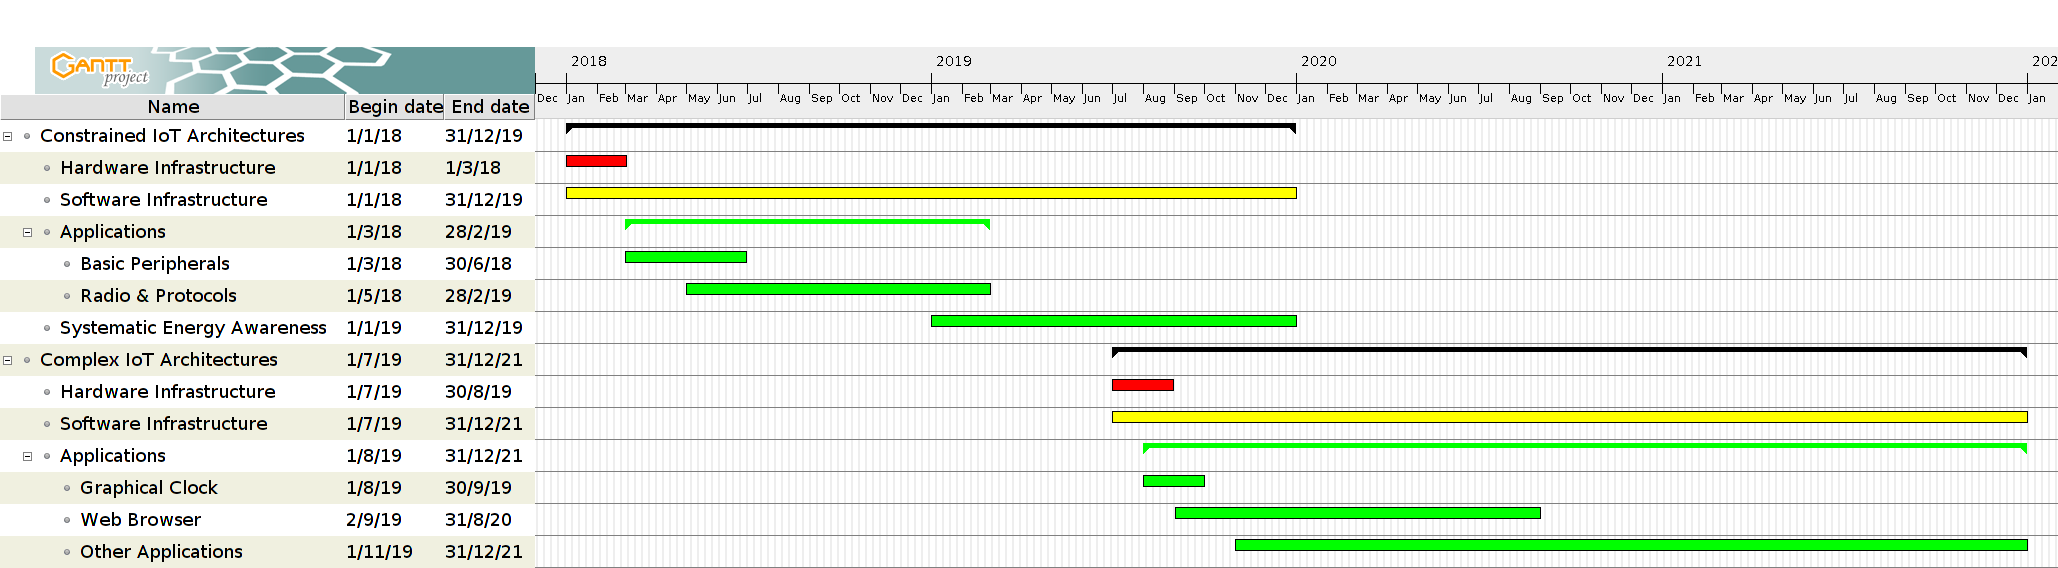
\includegraphics[width=\columnwidth]{serra-big}
    \caption{Project timeline
        \label{fig.timeline}
    }
\end{sidewaysfigure}

\section{RESOURCES}

For the period of 3 years, we will require a budget of R\$345k:
\begin{itemize}
    \item R\$300k for staff payment (87\%),
    \item R\$20k for equipment (6\%), and
    \item R\$25k for publication and travel costs (7\%).
\end{itemize}

\subsection{The Team}

Most of the resources will be employed in research staff consisting
of undergraduate, MSc, and PhD students.
%
The quality and long-term commitment of the students is paramount for the
success of the project.
%
For this reason, we want to offer a salary compatible with the industry, which
is considerably larger than typical research scholarships.

\begin{description}
\item[Proponent]
The proponent will work in all project fronts: managing the resources and
staff, writing papers and supervising students, and working on the technical
challenges of the project.
\item[Advisors]
The proponent is an associate professor at UERJ and a member of the LabLua%
\footnote{LabLua: \url{http://www.lua.inf.puc-rio.br/}.}
at PUC-Rio.
The advisors are experienced researchers from UERJ and PUC-Rio in the field of
programming languages, distributed systems, and wireless sensor networks.
They will support the academic duties, such as prospecting and supervising
students, writing papers, and helping on the general project guidelines.
\item[Research staff]
At the beginning of the first year, we will appoint two students to join the
project full time:
    one early-stage PhD student
and
    one MSc student or late-stage undergraduate student.
Every six months, we plan to add a new member to the staff until we reach a
limit of 6 students (consisting of 2 or 3 PhD students).
The PhD students will work with the software infrastructure and the other
students with the applications.
We also expect that the PhD students will work on academic papers and
take advantage of the project in their thesis.
Considering an average of 4 students during the whole project with and an
average salary of R\$2k, we expect to spend around R\$300k with payments.
\end{description}

\subsection{Infrastructure and Equipment}

The required equipment is divided between support for the research staff (printer and
laptops) and the project embedded systems (Arduino, Beagle Black, etc.):
\newline

%{%\linespread{0.5}
{\renewcommand{\arraystretch}{0.8}
\begin{tabular}{ | l | r | r | r | }
\hline			
EQUIPMENT       & PRICE & QTD   &   TOTAL   \\
\hline  
Laser printer   & 3000  &   1   &   3.000    \\
Laptop          & 4000  &   3   &  12.000    \\
Arduino kits    &  200  &   5   &   1.000    \\
Sensors \& radios & -   &   -   &   2.000    \\
Beagle Black    &  600  &   2   &   1.200    \\
Beagle Display  &  400  &   2   &     800    \\
\hline  
                &       &       &  R\$20k \\
\hline  
\end{tabular}
\newline
}

We expect that half of these resources will be acquired at the beginning of the
project.
The other half will be acquired gradually during the course of the 3 years.

\subsection{Publication and Travel Costs}

Our goal is to publish our results on international journals in the field of
embedded systems and sensor networks, such as \emph{ACM TECS} and \emph{ACM TOSN}.
%
However, the process to publish a paper in a journal may take longer than a year after
the submission.
For this reason, we also intend to publish partial results in conferences.

During the 3 years, we plan to attend two Brazilian conferences (e.g.,
\emph{SBRC}),
%and the \emph{Brazilian Symposium on Computing Systems Engineering (SBESC)}),
and one prestigious international conference (e.g., \emph{ACM SenSys}),
These venues are important to cultivate future cooperation with other research
groups.
For the Brazilian conferences, we will support 2 participants, and for the
international conference, only 1 participant.
%
Using the CNPq travel grants as a reference, attending a national conference
costs around R\$3k (including travel and accommodation for 3 days), while a 
international conference costs around US\$4k (including travel and
accommodation for 5 days).
Considering the two Brazilian conferences with two participants each, and one
international conference with one participant, the total travel costs for the
3-year period will be around R\$25k.

\begin{comment}
\section{CONCLUSION}

TODO

- conslidated research
- some steps already done
- we need human resources

realistic research
    - academic results
    - but also an open-source publicly available language that people can download and use
        - already available
        - all publics: research, hobbyists, students

TODO: long-term research
    - 8 years in the same project
\end{comment}

\newpage
\bibliographystyle{abbrv}
\bibliography{serra,my}
\end{document}
